\autsubsection{Sputtering Drilling}{Paul Connetable}

\subsubsection{Sputtering physics and research on sputtering on water ice}

The concept of sputtering is to send particles with a high kinetic energy on a solid, in order to eject the surface particles of the solid. Generally, the particles sent on the solid are ions, but it can be any atom. It is the energy exchange between the incoming particle and the surface molecules which eject these particles. In order to be ejected, the energy brought to the solid surface must exceed the binding energy of its molecules. A single particle sent can eject several atoms or particles at once, and is called the sputter yield. The sputter yield depends on the ion incident angle, its mass, its velocity, and the mass and the binding energy of the solid atoms. Some research about sputtering on water ice has been made in \cite{baragiola2003sputtering}.
In this research, the sputtering yield of water ice has been measured under several conditions, and for several types of ions, and several very interesting results have been obtained:
\begin{itemize}
    \item {The sputtering yield of water ice is constant below 100K for $O_{+}$, $AR_{+}$ and $HE_{+}$ ions, as shown in Figure \ref{sputtering30kev}}
    
\begin{figure}[htb]
\begin{center}
%\fbox{
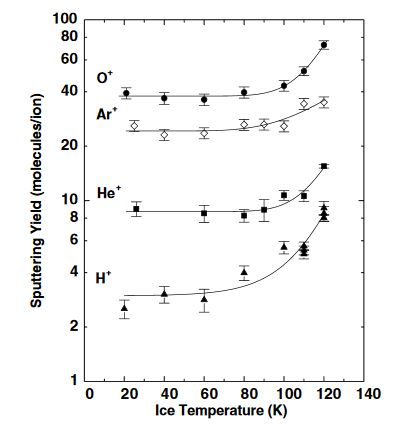
\includegraphics{Paul/sputtering30kev.JPG}
%}
\end{center}
\caption{Influence of ice temperature on the sputtering yield}
\label{sputtering30kev}
\end{figure}

    \item {The sputtering yield of water ice is dependent on the fluence, (i.e. the concentration of ions sent on the ice surface per surface unit) for $O_{+}$ ions only, among the different ions tested. It increases from 11 to 14 molecules as shown in Figure \ref{sputteringfluence}}
    
\begin{figure}[htb]
\begin{center}
%\fbox{
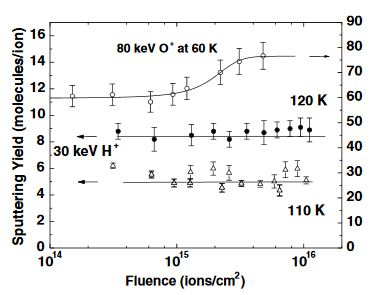
\includegraphics{Paul/sputteringfluence.JPG}
%}
\end{center}
\caption{Influence of fluence on the sputtering yield}
\label{sputteringfluence}
\end{figure}

    \item {The influence of the incoming ion's energy on the sputtering yield is shown in Figure \ref{sputteringenergy} below. One can observe that thresholds appear for $O_{+}$ and $H_{+}$ ions in the displayed energy interval.}
    
\begin{figure}[htb]
\begin{center}
%\fbox{
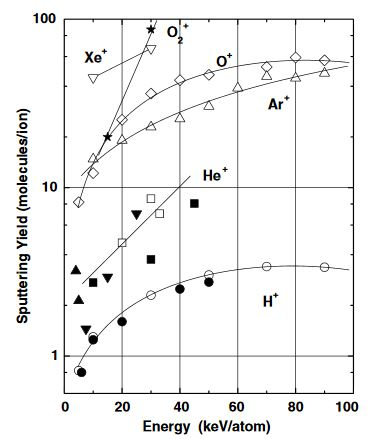
\includegraphics{Paul/sputteringenergy.JPG}
%}
\end{center}
\caption{Influence of the incoming ion energy on the sputtering yield}
\label{sputteringenergy}
\end{figure}

\end{itemize}

\subsubsection{Conclusion on the metod}

These results allow a quick calculation on the energy needed to drill through a certain depth of ice. To erode 1 liter of ice at 60K, the total energy needed by sputtering is of approximately $10^{44}~kJ$. As a comparison, the energy needed to evaporate one liter of ice is of $3~\times10^{3}~kJ$. It is to be expected that the total energy required to just melt and evaporate ice is way smaller than the energy needed to erode it by sending ions on it, but these results show an enormous difference.

Sputtering drilling has other drawbacks for our mission:
\begin{itemize}
\item{this technique would create a contamination of the middle~;}
\item{using this technique would mean to bring a material reserve, which would be used to sputter the ice. This reserve would weight a lot.}
\end{itemize}

Actually, sputtering has only been researched on very thin layers of ice. In \cite{baragiola2003sputtering}, the maximum thickness of ice tested was of 250 nm.This method is not the best to drill holes, but is rather commonly used to erode surfaces and deposit thin layers of material on manufactured products. this is why this method is not the one chosen on our mission on Europa.